%! TeX program = xelatex
\documentclass[12pt]{beamer}
\usepackage{fontspec}
\setmainfont{QTBookmann}
\usepackage{polyglossia}
\usepackage{xcolor}
\usepackage{graphicx}
\setdefaultlanguage{spanish}

% Usar tu tema ENCOM
\usepackage{BeamerENCOMTheme}

\title{Análisis Predictivo de Precios de Vivienda}
\author{[Tu Nombre]}
\date{\today}


\newcommand{\bgimg}[1]{
  \setbeamertemplate{background}{%
    \vbox%
      to \paperheight{\vfil\hbox%
        to \paperwidth{\hfil%
      \includegraphics[width=\paperwidth, height=\paperheight]{#1}
      \hfil}\vfil}
  }
}


\begin{document}

% Fondo para la portada
\bgimg{fondo.png}
\begin{frame}
  \centering
  \vspace{1cm}
  {\LARGE\color{white} \textbf{Análisis Predictivo de Precios de Vivienda}}
  
  \vspace{0.5cm}
  {\large\color{yellow} Manejo de Outliers con Métodos Avanzados}
  
  \vspace{1cm}
  {\color{white} [Tu Nombre]}
  
  \vspace{0.3cm}
  {\color{white} \today}
\end{frame}

% Fondo difuminado para el contenido
\bgimg{blured.png}

\begin{frame}
\frametitle{Introducción}
\begin{itemize}
\item Outliers afectan modelos predictivos en datos inmobiliarios
\item Adaptación de métodos de Alkan et al. (2024)
\item Regresión de Cox → Precios de vivienda
\end{itemize}
\end{frame}

\begin{frame}
\frametitle{Metodología}
\begin{itemize}
\item Dos escenarios comparativos:
\begin{itemize}
\item Datos crudos sin tratamiento
\item Datos con imputación múltiple
\end{itemize}
\item Algoritmos evaluados:
\begin{itemize}
\item Regresión Lineal, Ridge, Lasso
\item Random Forest (mejor resultado)
\end{itemize}
\end{itemize}
\end{frame}

\begin{frame}
\frametitle{Resultados - Comparación de Modelos}
\centering
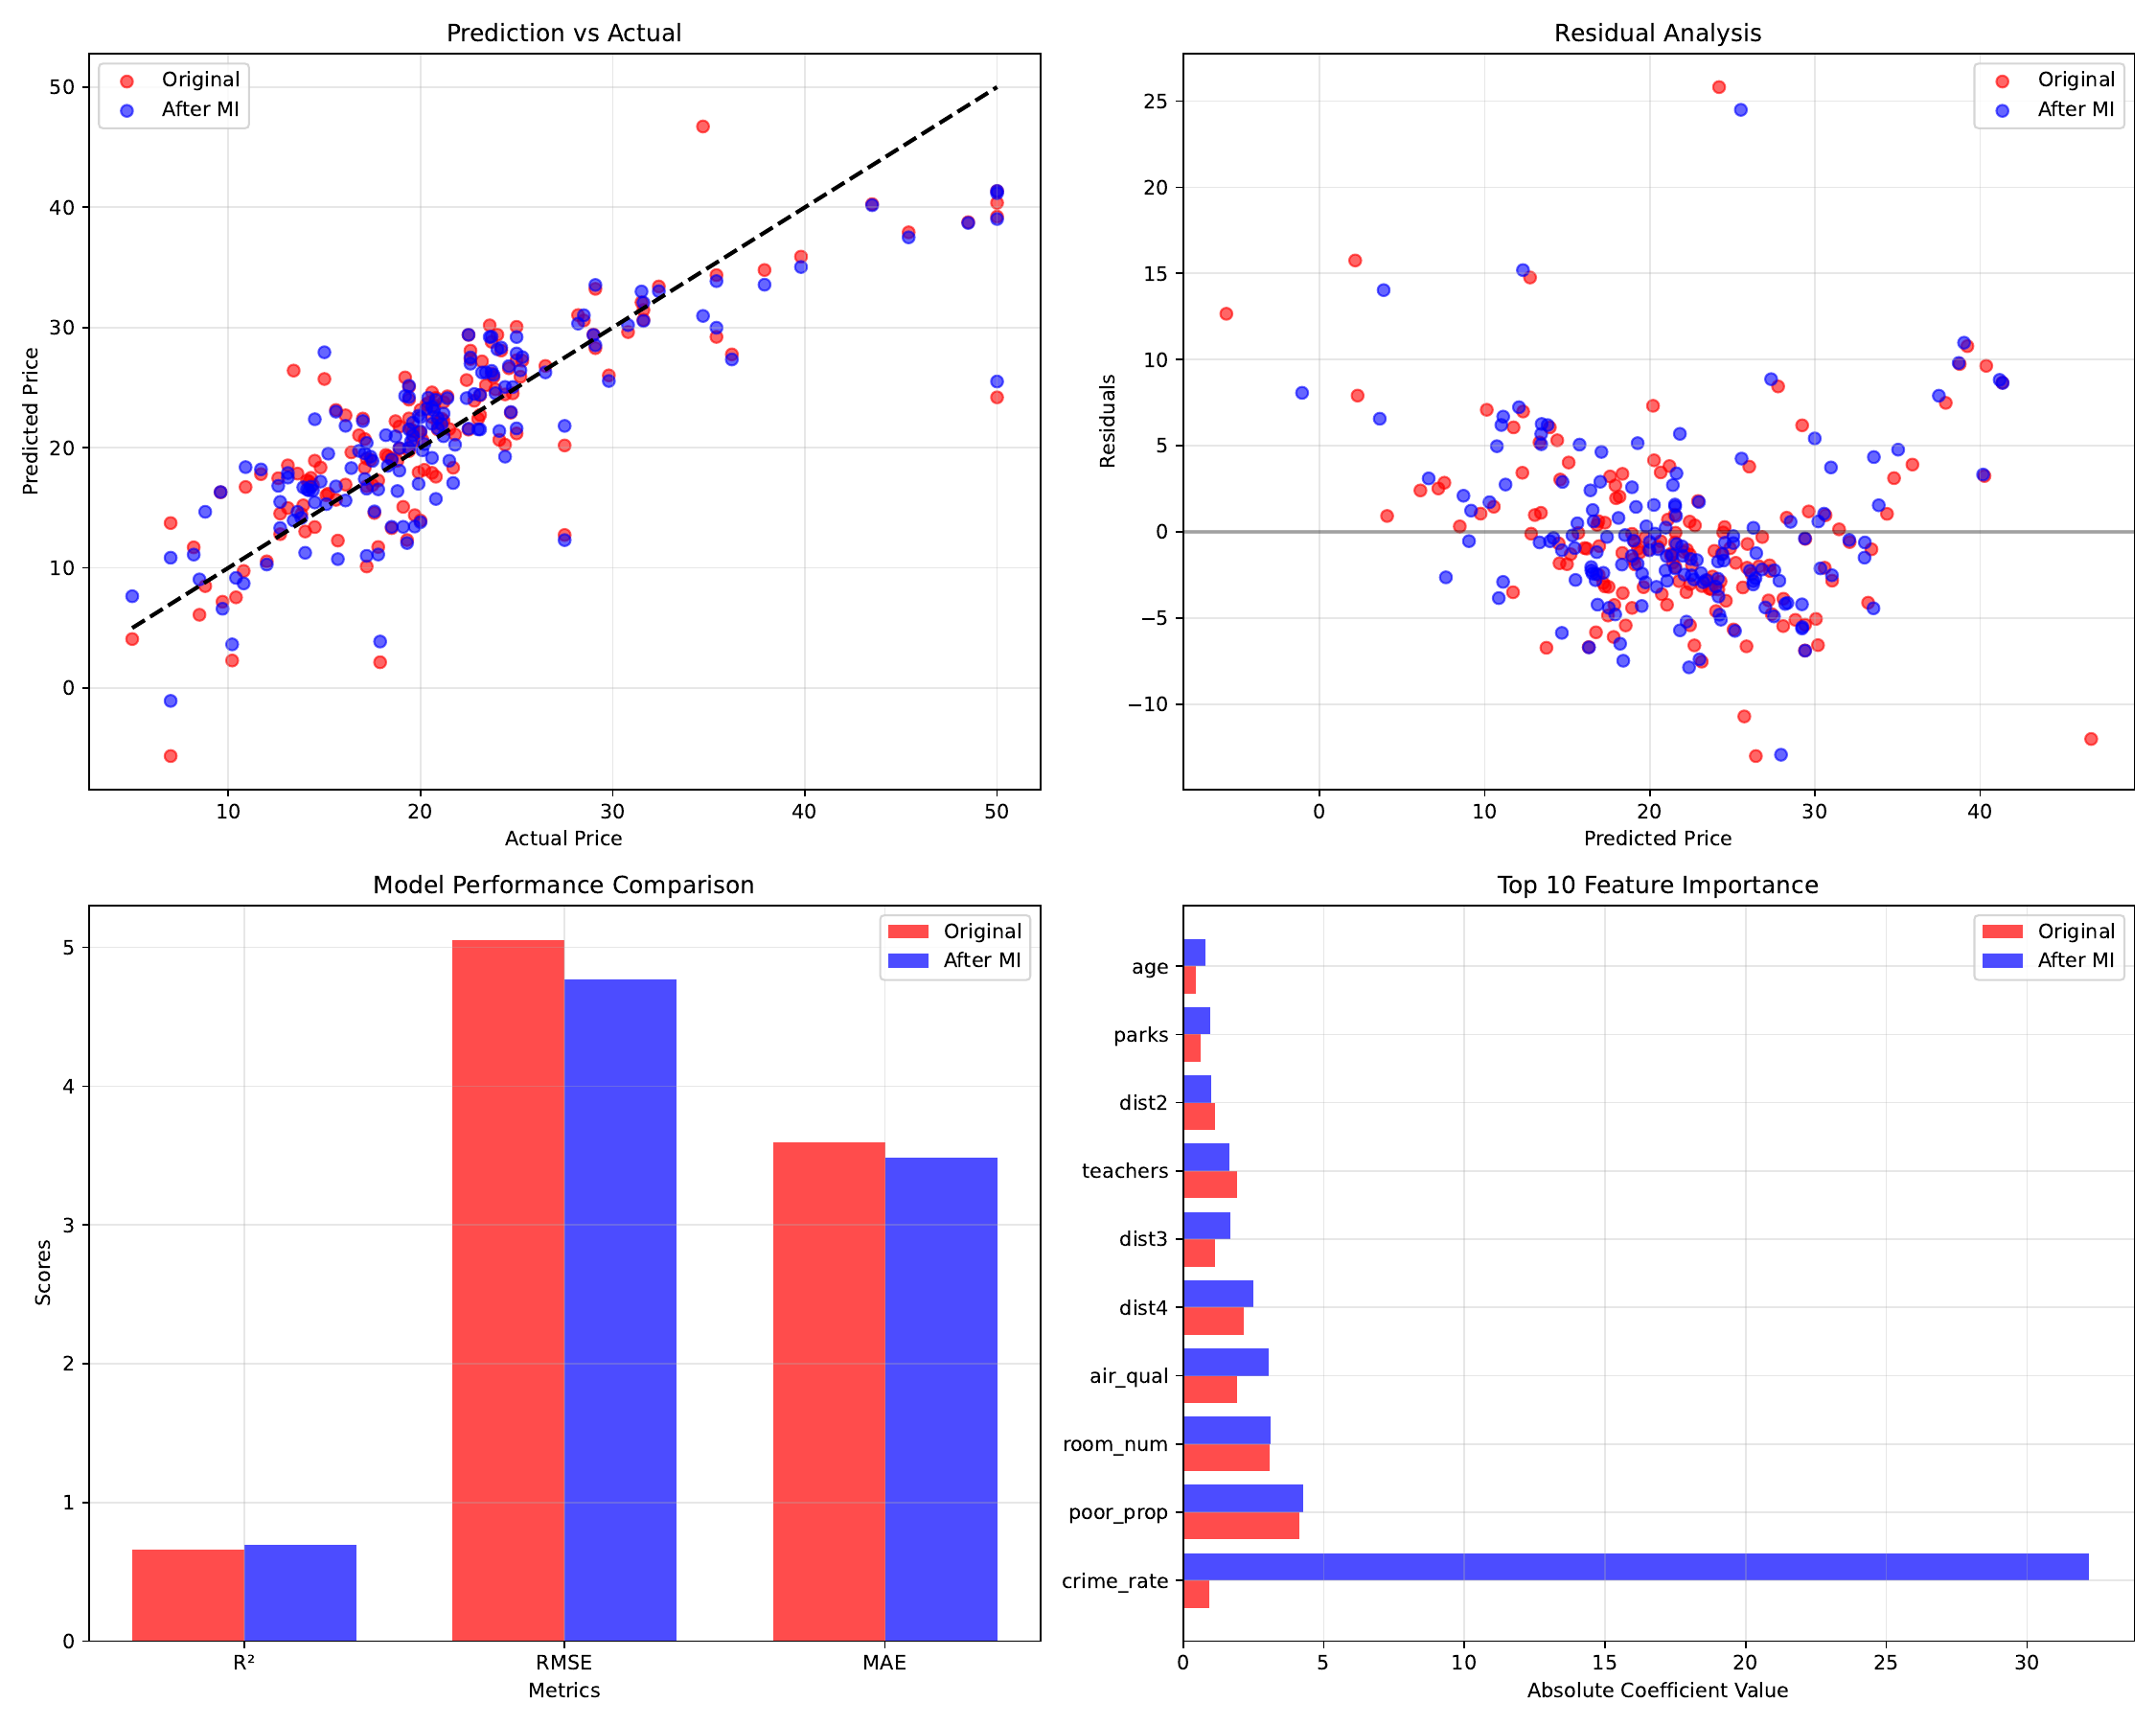
\includegraphics[width=0.9\textwidth]{regression_comparison-1.png}
\end{frame}

\begin{frame}
\frametitle{Resultados - Métricas}
\centering
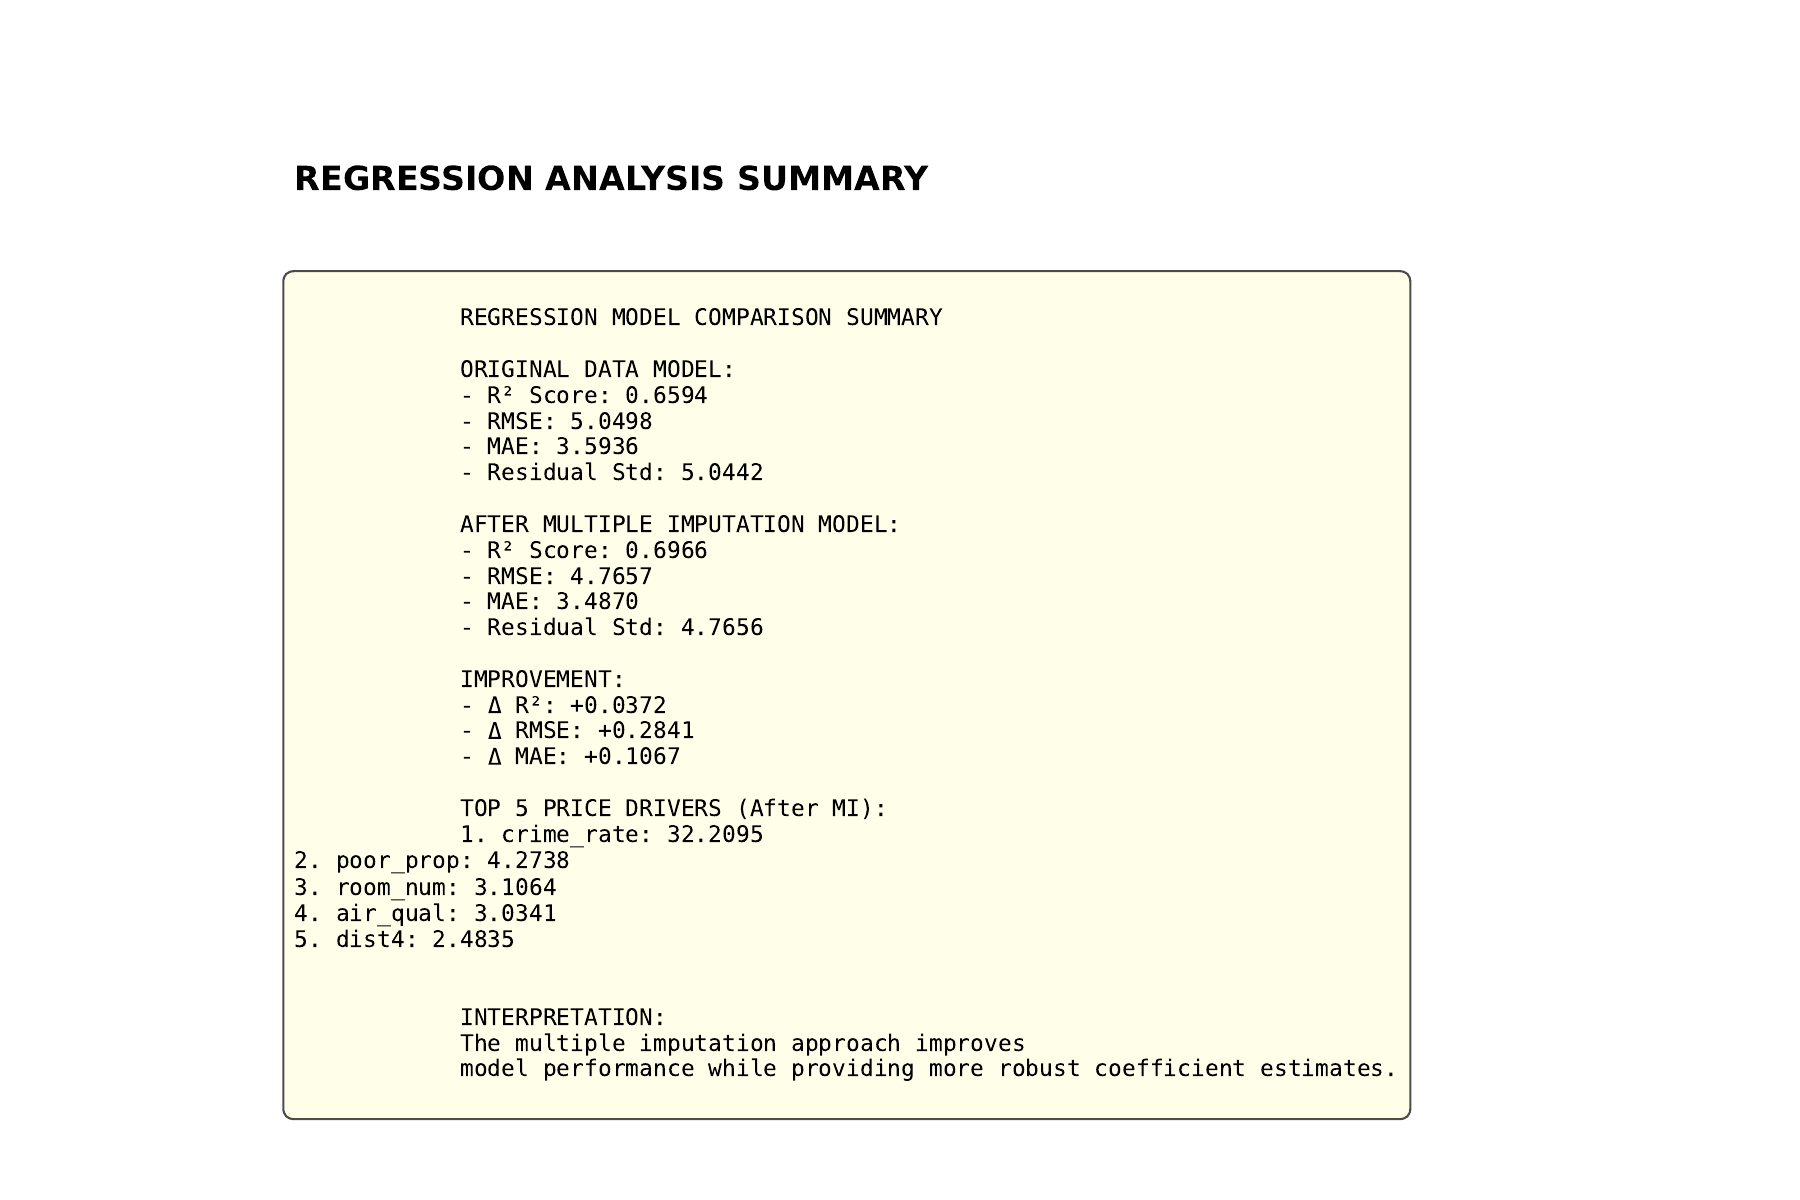
\includegraphics[width=0.9\textwidth]{regression_comparison-2.png}
\end{frame}

\begin{frame}
\frametitle{Resultados - Predicción vs Real}
\centering
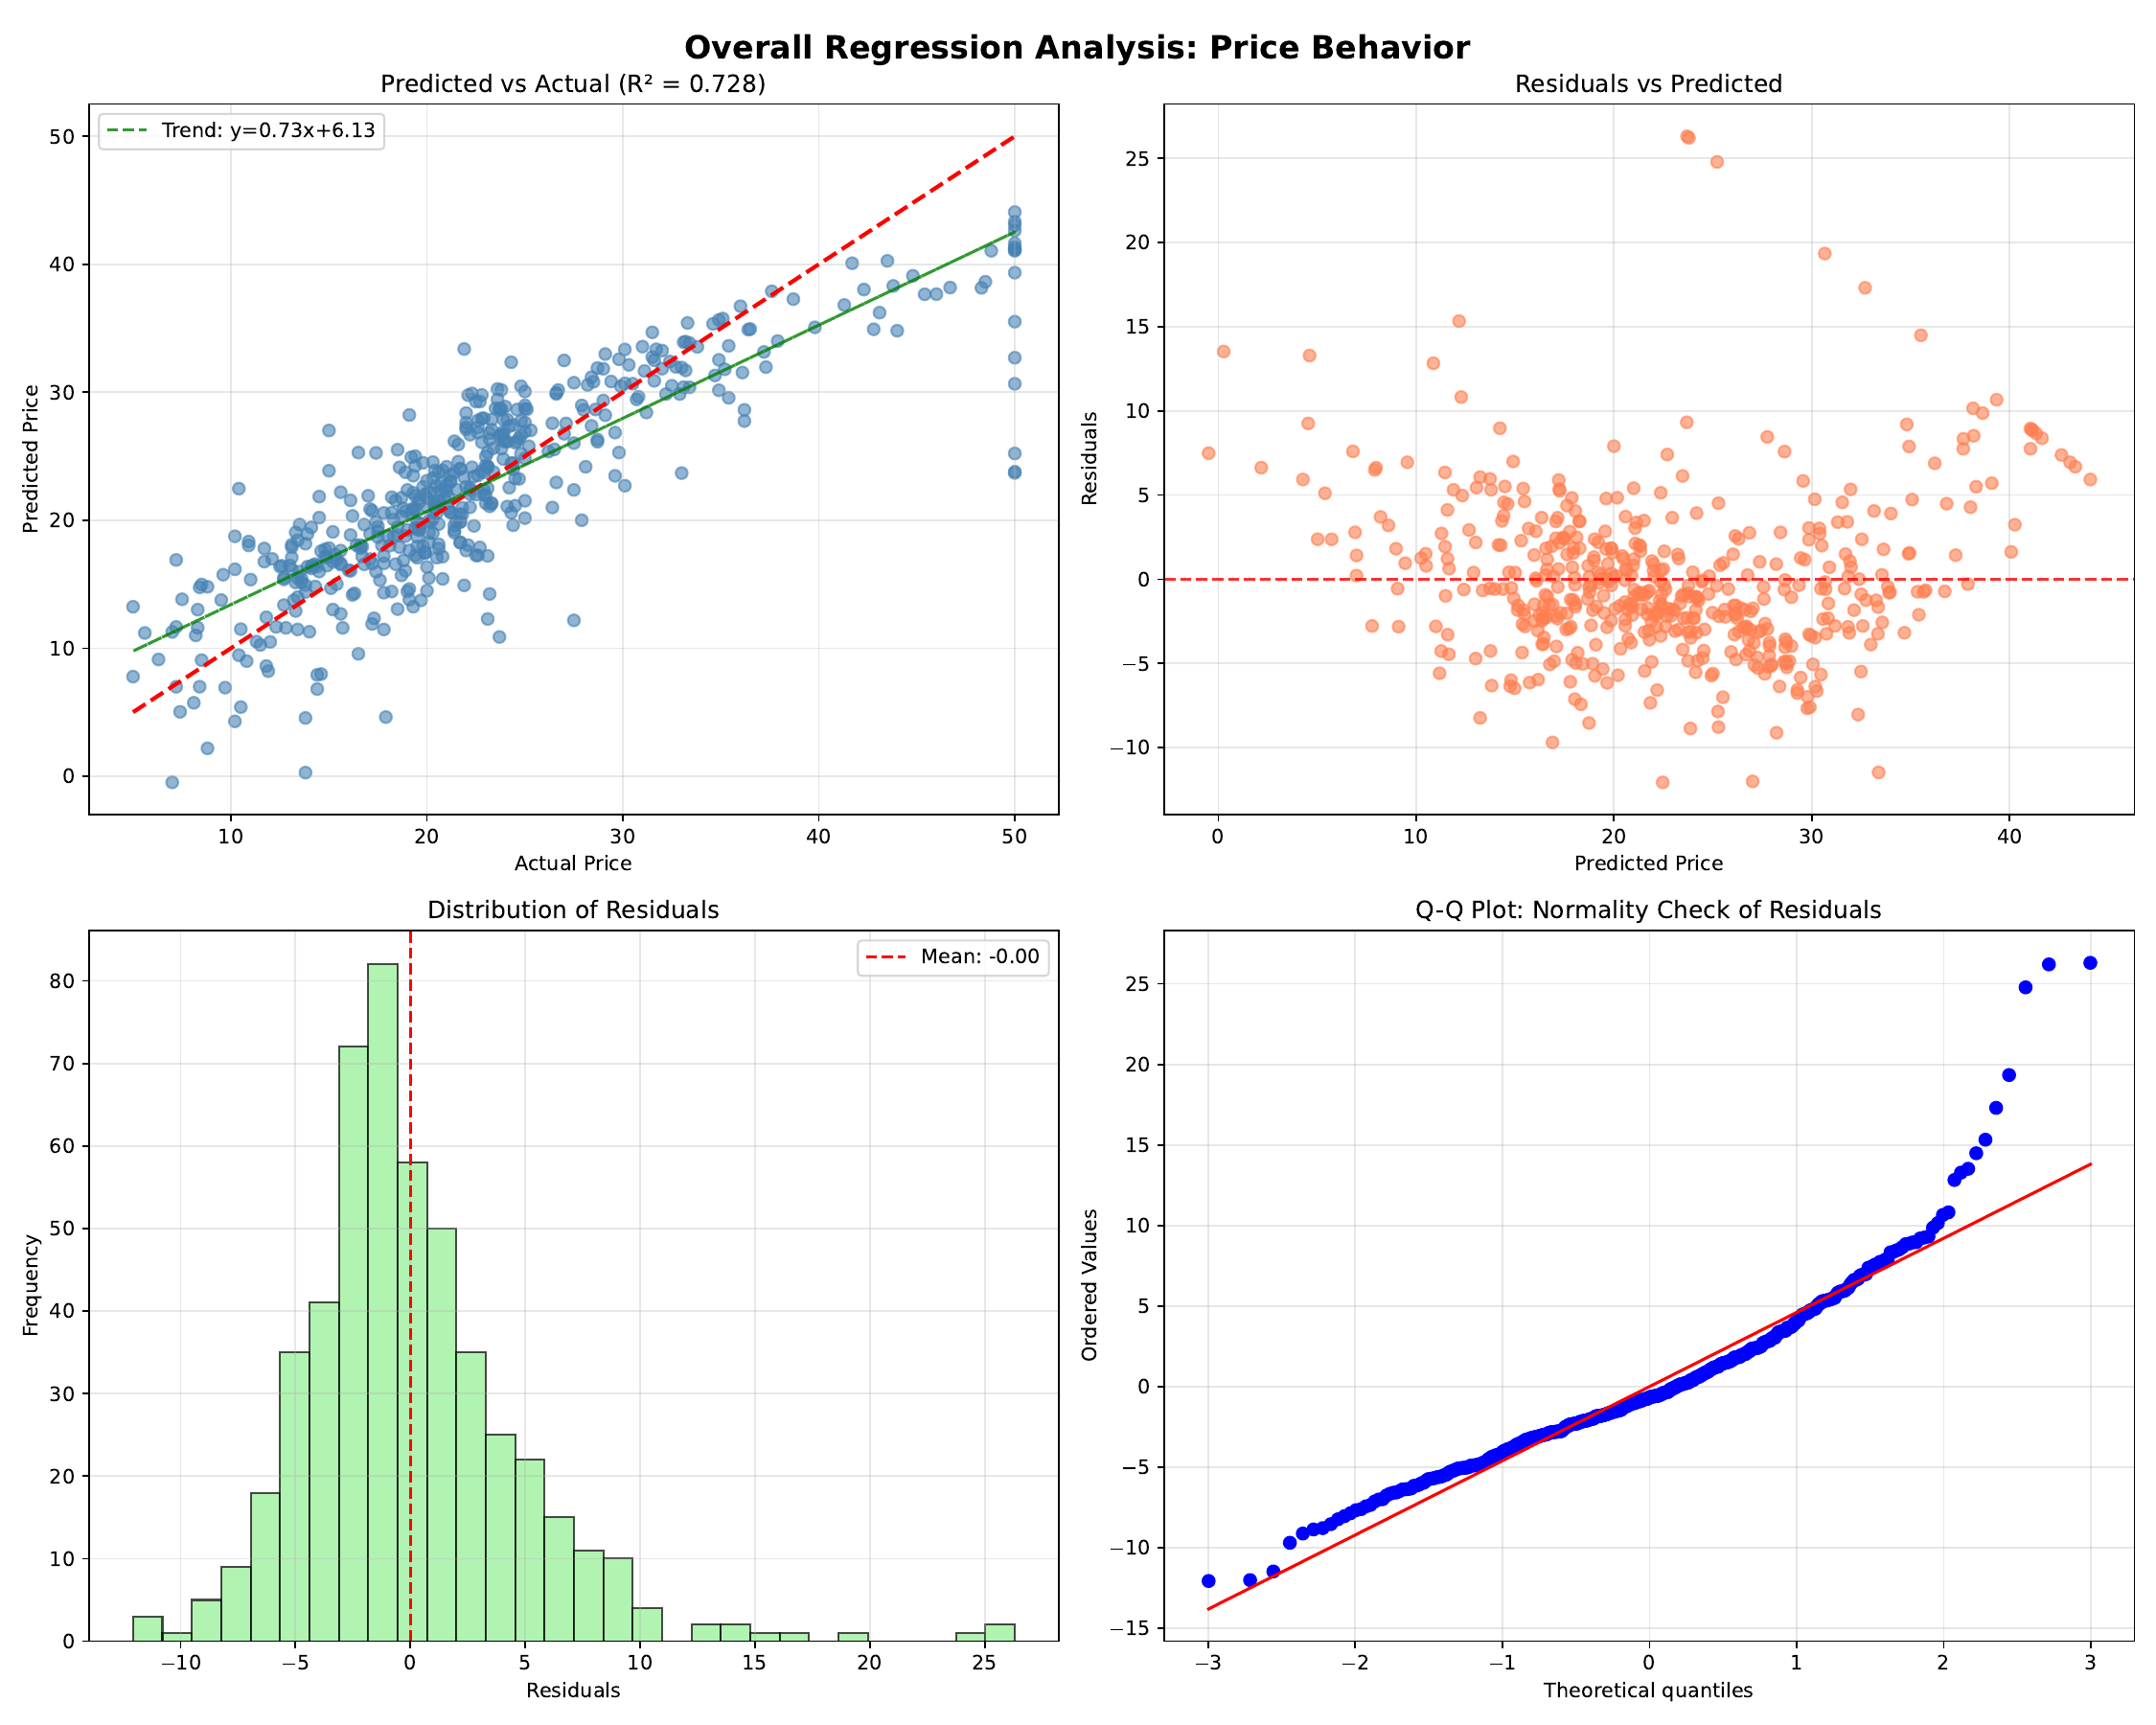
\includegraphics[width=0.9\textwidth]{regression_analysis-1.png}
\end{frame}

\begin{frame}
\frametitle{Resultados - Variables Importantes}
\centering
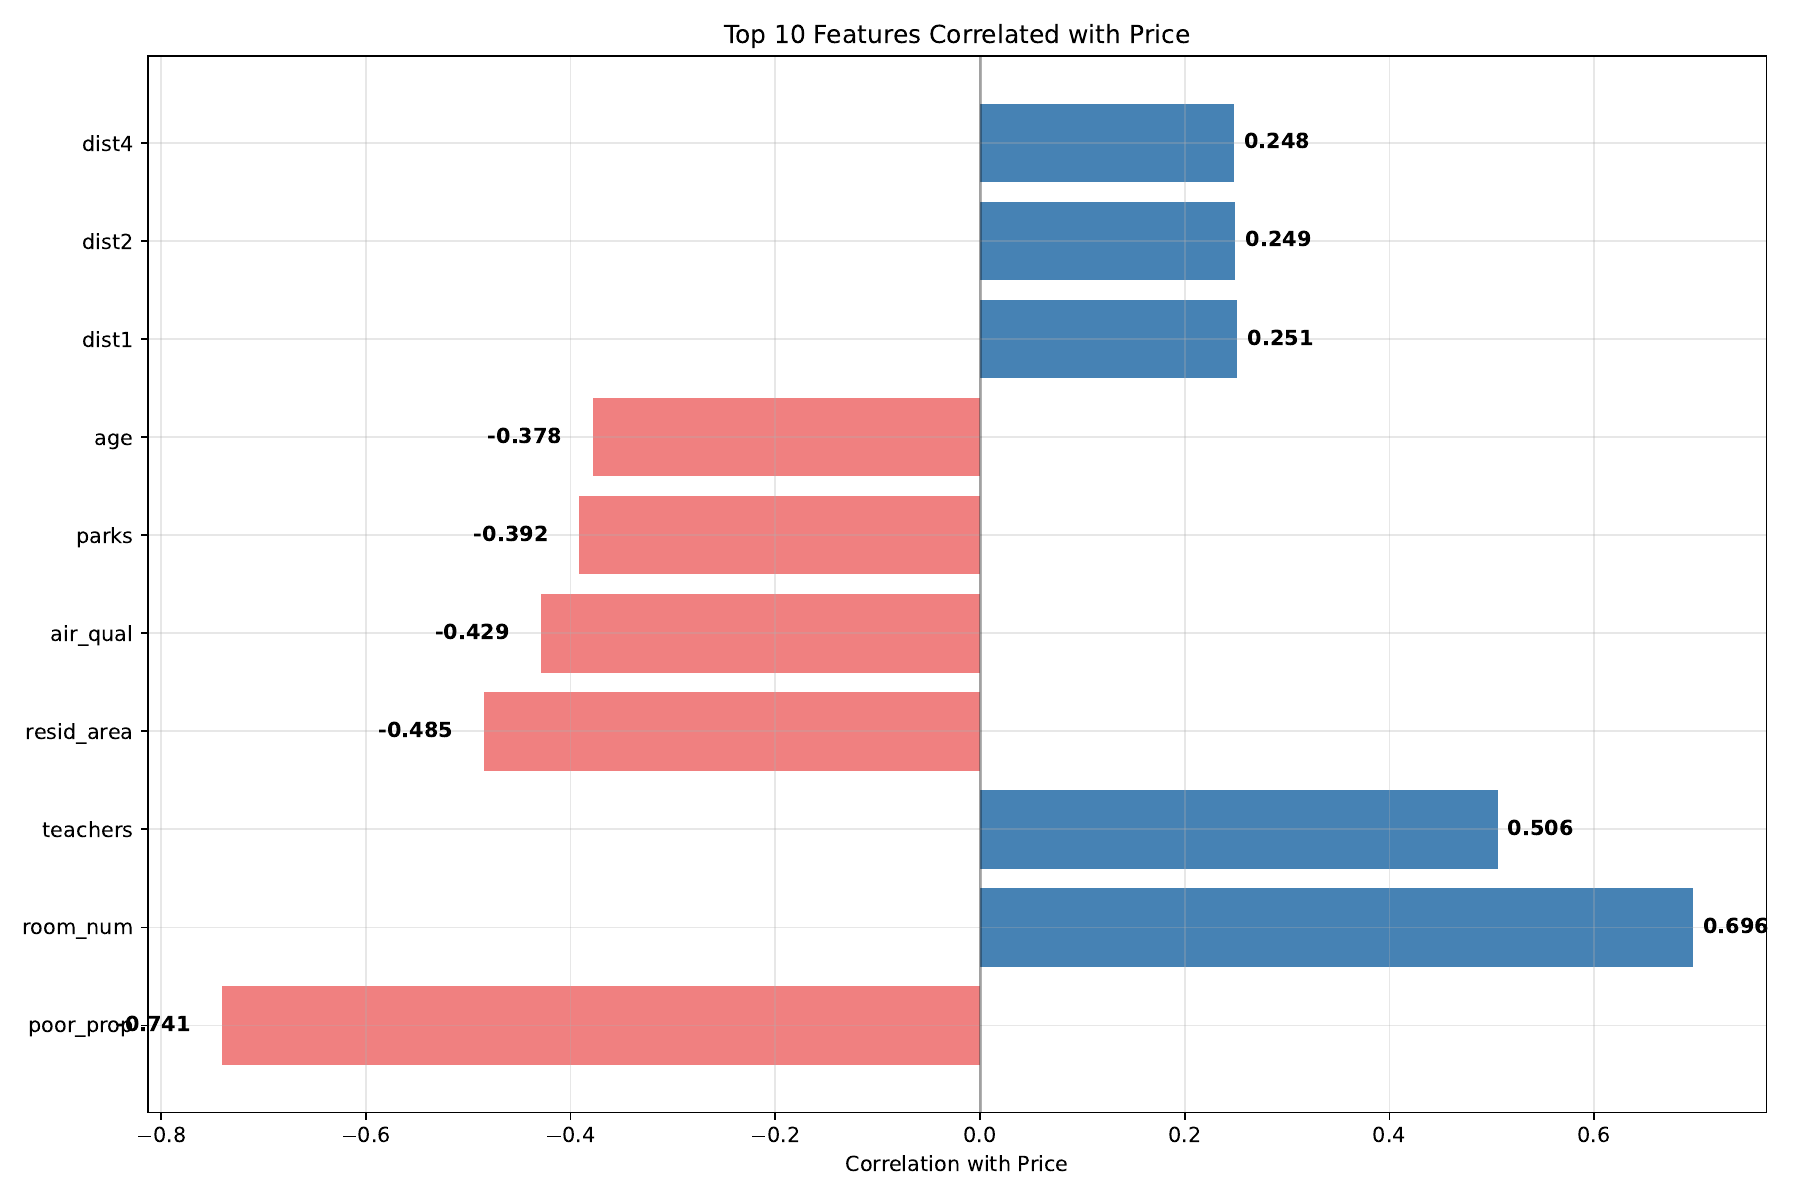
\includegraphics[width=0.9\textwidth]{price_behavior_quick-2.png}
\end{frame}

\begin{frame}
\frametitle{Resultados - Análisis de Residuales}
\centering
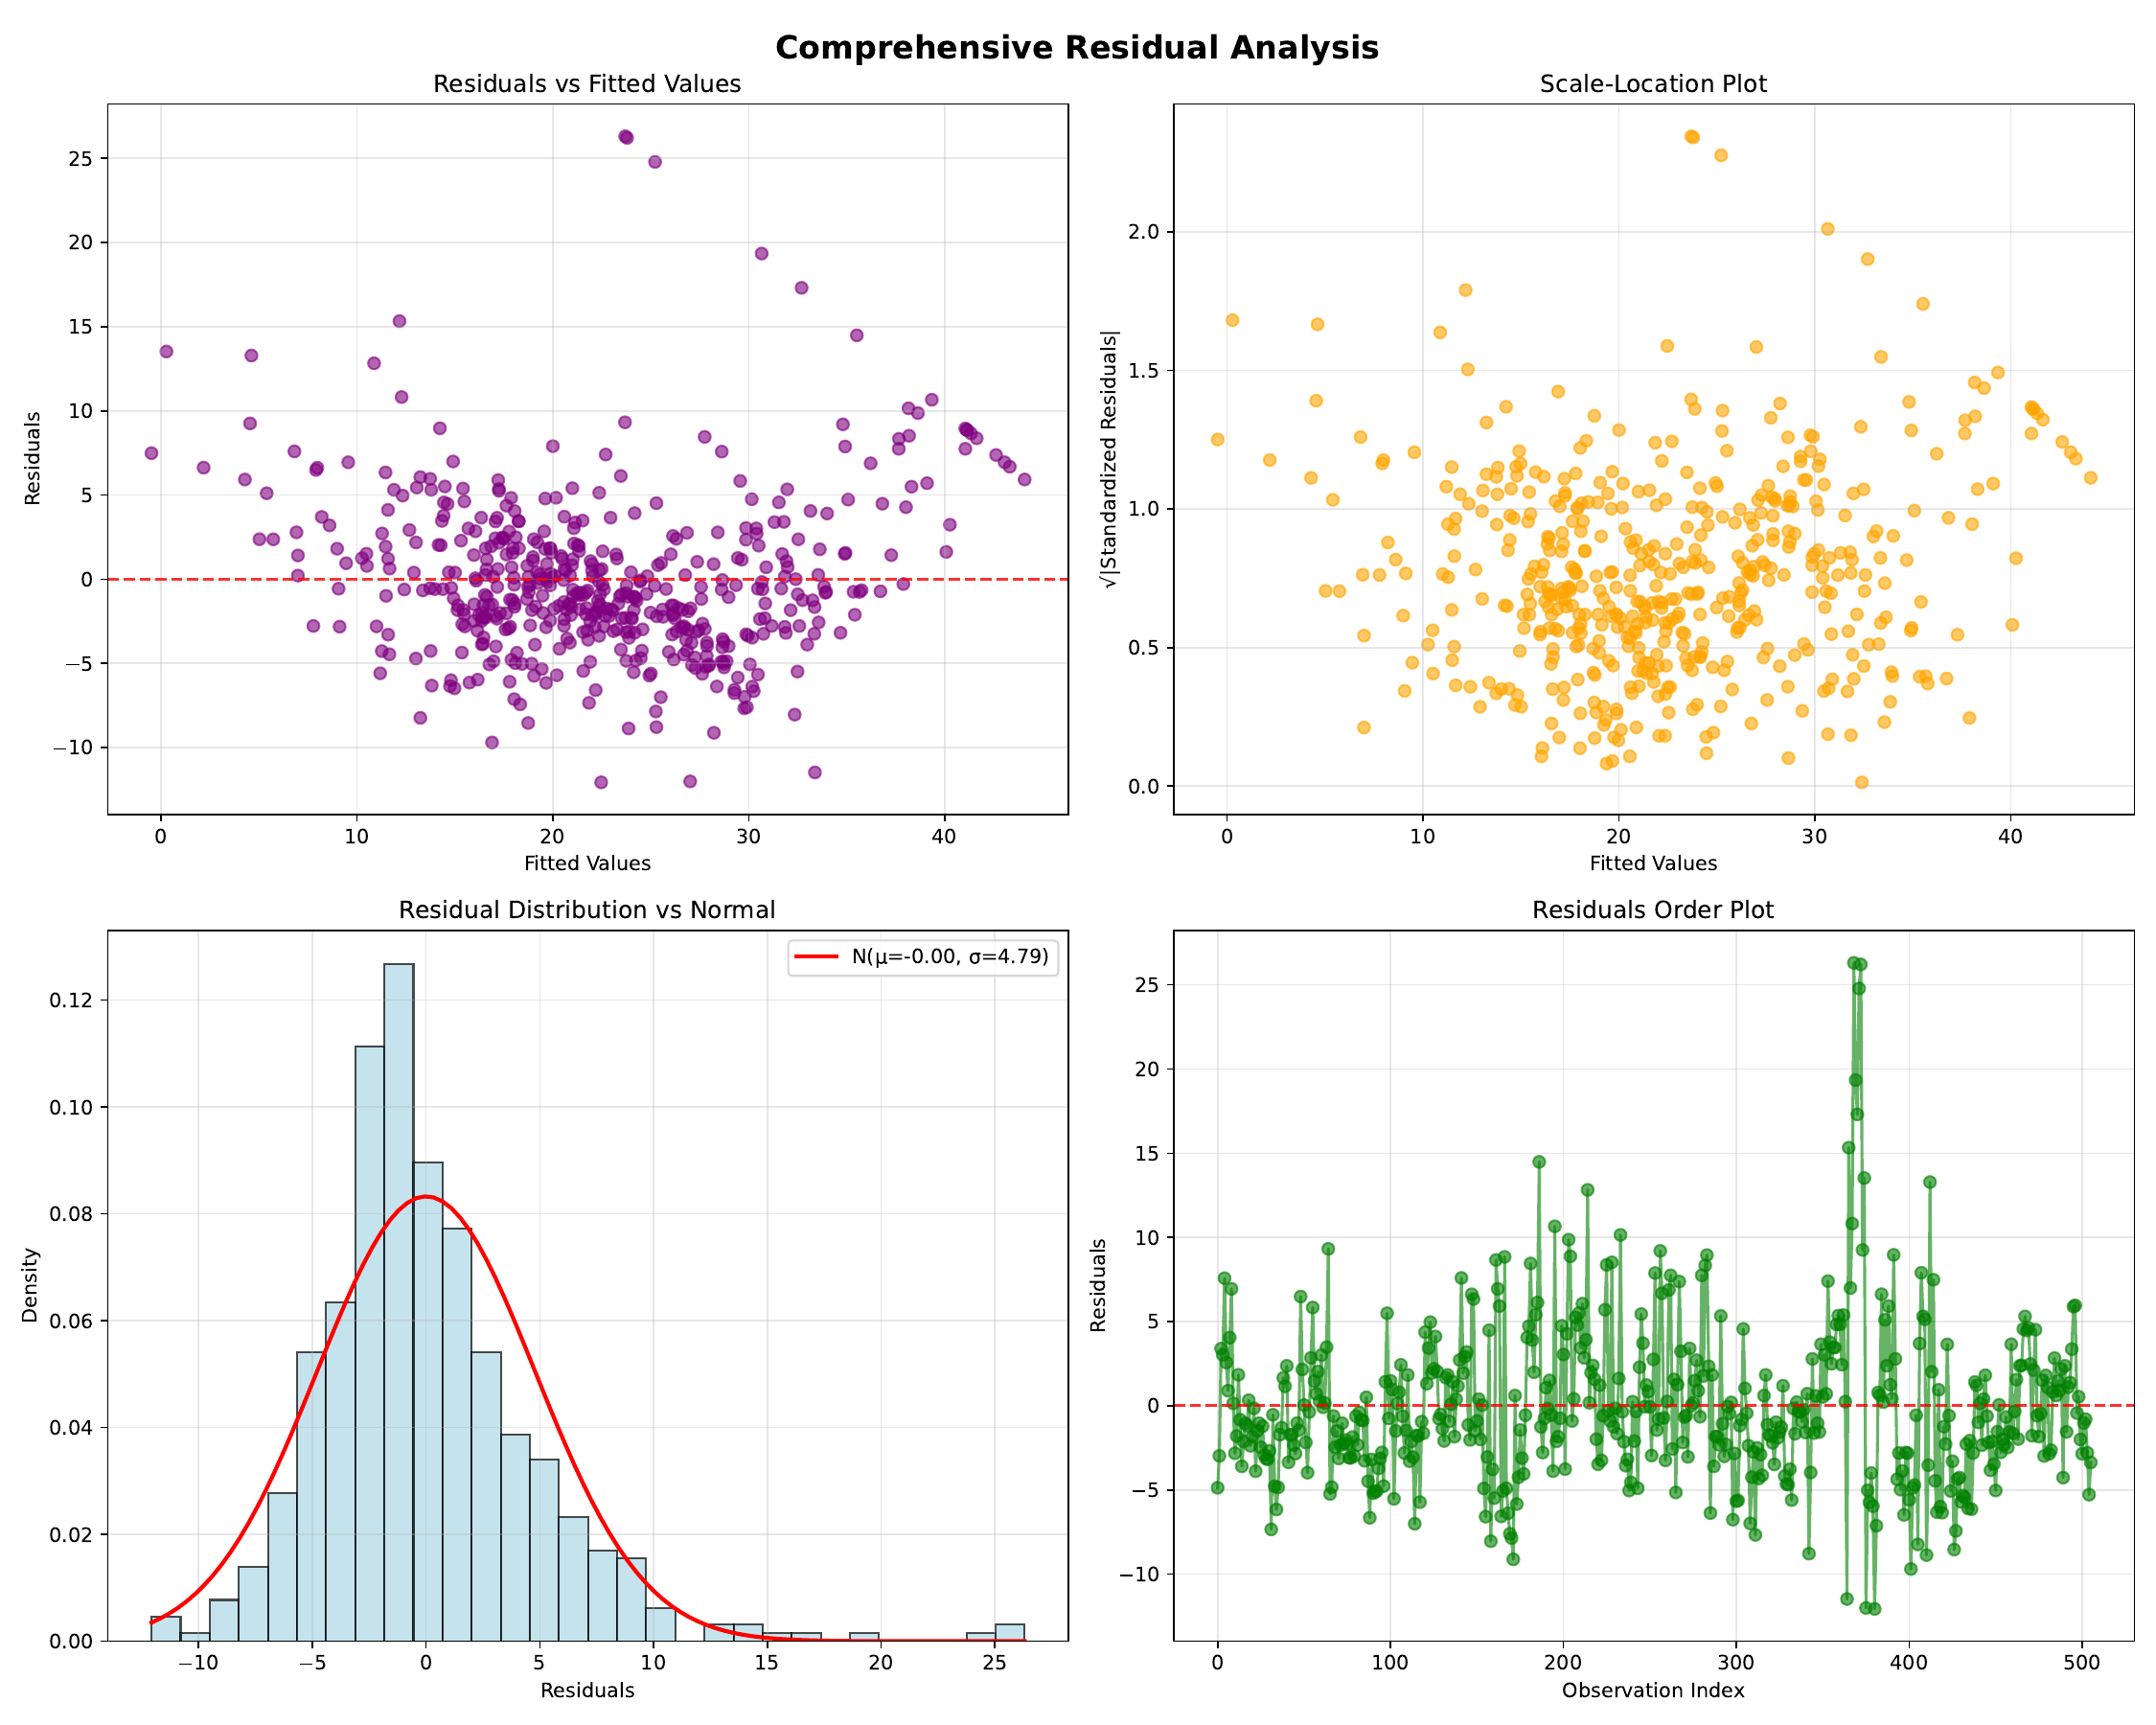
\includegraphics[width=0.9\textwidth]{regression_analysis-3.png}
\end{frame}

\begin{frame}
\frametitle{Resultados - Importancia de Variables}
\centering
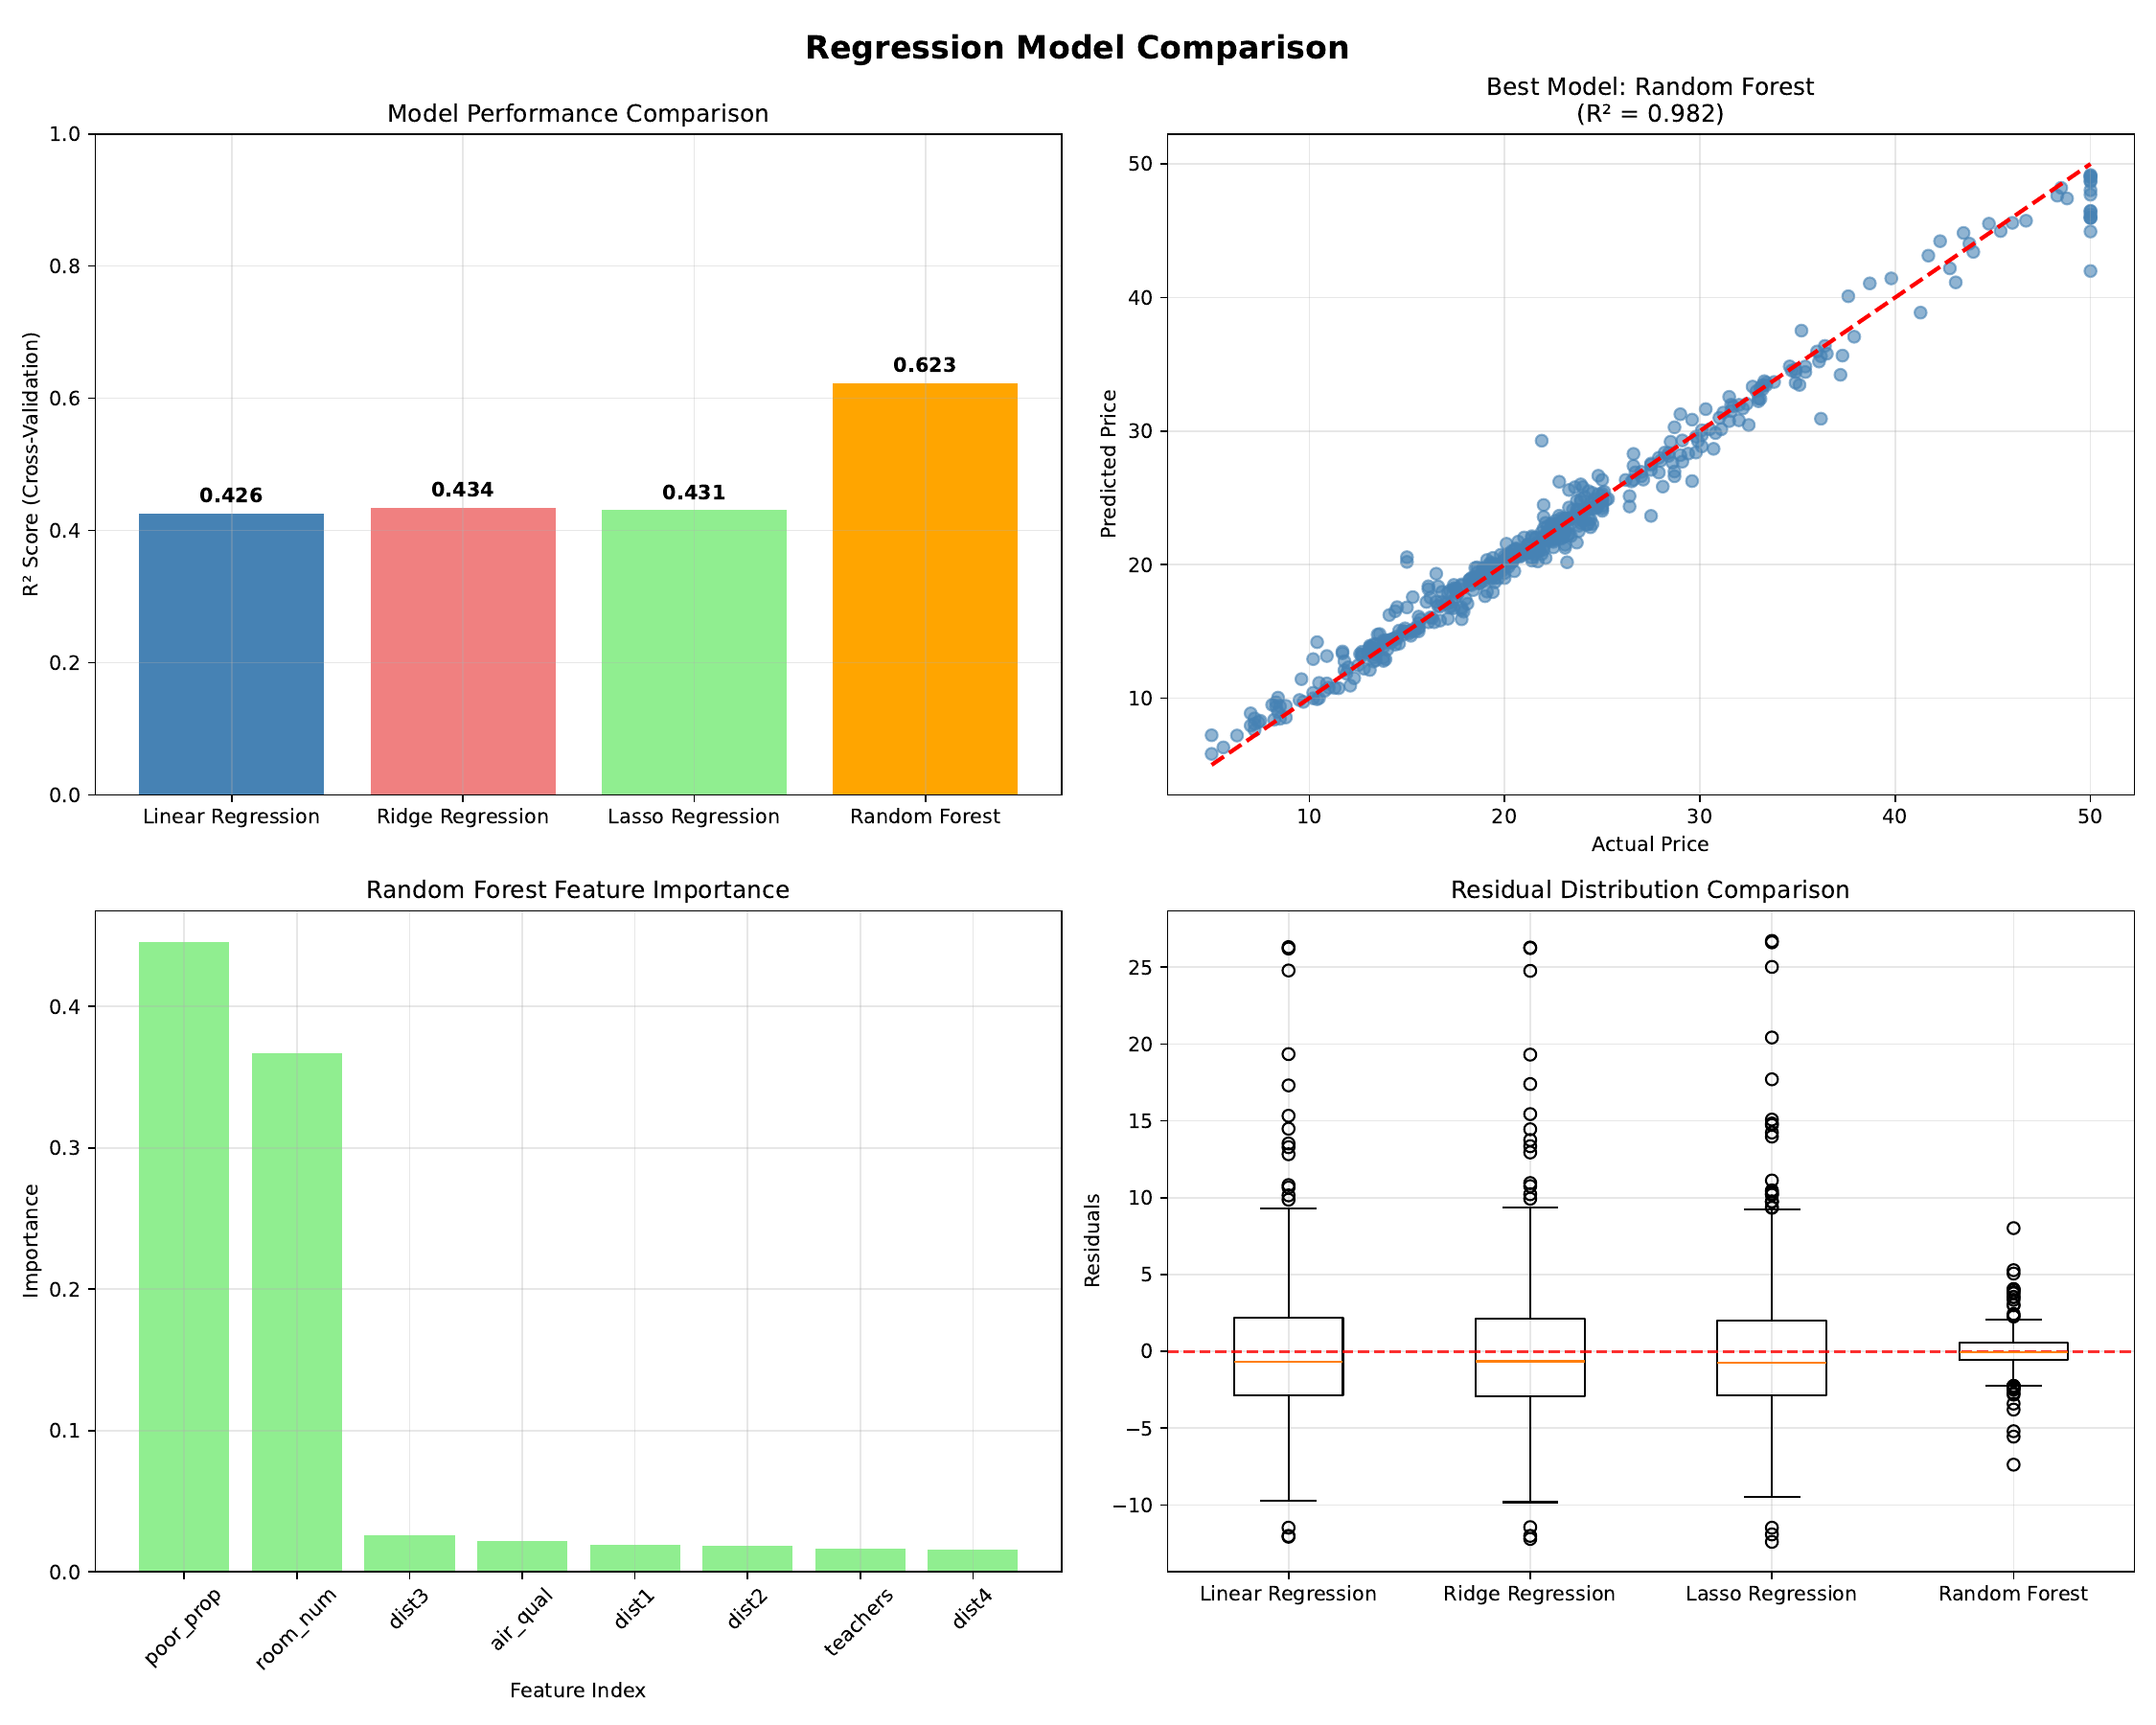
\includegraphics[width=0.9\textwidth]{regression_analysis-5.png}
\end{frame}

\begin{frame}
\frametitle{Conclusiones}
\begin{itemize}
\item Imputación múltiple mejora R² en 0.0372
\item Random Forest: mejor modelo (R² = 0.982)
\item Variables contextuales más importantes que físicas
\item Método efectivo para manejo de outliers
\end{itemize}
\end{frame}

\end{document}
